\documentclass[11pt, a4paper]{article}

\usepackage[lang=en,grid=dark]{kufront}

\usepackage{tikz}
\usetikzlibrary{shapes,matrix,decorations.pathreplacing}
\usepackage[utf8]{inputenc}
\usepackage[T1]{fontenc}
\usepackage{amsmath, amssymb}
\usepackage{amsthm}
\usepackage{mathtools}
\usepackage{amsfonts}
\usepackage{pdfpages}
\usepackage{gauss}
\usepackage{fancyvrb}
\usepackage{hyperref}
\usepackage{graphicx, import}
\usepackage{subcaption}
\usepackage{url}
\usepackage{float}
\usepackage[bottom]{footmisc}
\usepackage{color}
\usepackage{adjustbox}
\usepackage{changepage}
\usepackage{longtable}
\usepackage{stmaryrd}
\usepackage{multirow}
\usepackage{wrapfig}
\usepackage{booktabs}
\usepackage{xfrac}
\usepackage{tabularx}
\usepackage{subcaption}

\usepackage[group-separator={,}]{siunitx}
\sisetup{group-minimum-digits = 3}

% \abs{} command
\DeclarePairedDelimiter\abs{\lvert}{\rvert}
\makeatletter
\let\oldabs\abs
\def\abs{\@ifstar{\oldabs}{\oldabs*}}

% algorithms
\usepackage{algorithm}      % algorithm float environment
\usepackage[noend]{algpseudocode}  % from algorithmicx; no "end" on functions
\newcommand*\Let[2]{\State #1 $\gets$ #2}
\algnewcommand{\LineComment}[1]{\State \(\sslash\) #1}
\algrenewcommand\algorithmiccomment[1]{\hfill\(\sslash\) #1}
\algrenewcommand\algorithmicrequire{\textbf{Precondition:}}

% headers and footers
\usepackage{fancyhdr, lastpage}
\pagestyle{fancy}
\fancyhf{}
\renewcommand{\headrulewidth}{0pt}
\cfoot{Page \thepage\ of~\pageref{LastPage}}

% settings for lslisting
\definecolor{listinggray}{gray}{0.9}
\usepackage{listings}
\lstset{
  showtabs=false,
  showspaces=false,
  showstringspaces=false,
  columns=fixed,
  showstringspaces=false,
  extendedchars=true,
}

\lstdefinestyle{output-style}{
  basicstyle=\ttfamily\footnotesize,
  frame=tb,
}
\lstdefinestyle{output-top-style}{
  basicstyle=\ttfamily\footnotesize,
  frame=t,
  belowskip=0em,
}
\lstdefinestyle{output-no-style}{
  basicstyle=\ttfamily\footnotesize,
  aboveskip=0em,
  belowskip=0em,
}
\lstdefinestyle{output-bot-style}{
  basicstyle=\ttfamily\footnotesize,
  frame=b,
  aboveskip=0em,
}

% New commands
\newcommand{\eqdef}{\overset{\mathrm{def}}{=\joinrel=}}
\newtheorem{thm}{Theorem}

\title{Exact vertex-labeled distance oracles in static and dynamic planar graphs}
\subtitle{}
\author{Nikolaj Dybdahl Rathcke}
\project{Master's Thesis}
\supervisor{Supervisor: Christian Wulff-Nilsen}

\begin{document}
\begin{titlepage}
  \maketitle
\end{titlepage}

\pagestyle{plain}
\pagenumbering{roman}

\begin{abstract}
  TODO TODO TODO TODO TODO \\
  \\
  \begin{itemize}
    \item Expand introduction (introduce problem)
    \item Techniques
      \begin{itemize}
        \item Additively weighted Voronoi diagrams
      \end{itemize}
    \item Finish survey
      \begin{itemize}
        \item Planar case (dynamic)
      \end{itemize}
    \item Results
      \begin{itemize}
        \item Give $O(n^{1.5})$ space, $\text{poly}(\lg n)$ oracle (almost).
        \item Is it necessary to use klein/ddg for preprocessing in r-div?
        \item Other results? (FR-djikstra, dynamic version)
      \end{itemize}
    \item Concluding remarks and future works
    \item Appendices
  \end{itemize}
\end{abstract}

\newpage
\tableofcontents
\newpage

\pagestyle{fancy}
\pagenumbering{arabic}

\section{Introduction}\label{introduction}
Efficient algorithms on networks are playing an increasing important role today, and many
networks have structural properties that can be exploited to allow for much faster
algorithms than those in general graphs. One such class of networks are planar graphs, which have importance within
areas such as road transportation, computer vision and many more.. \\
As these networks can be quite large, one problem is constructing a compact \textit{distance
oracle}, which is a data structure that is able to either give exact or approximate
shortest paths between two nodes quickly while not taking up too much space. They were
introduced by Thorup and Zwick \cite{thorup2005approximate}. This problem has since been
extensively studied. However, a variant of this problem
was introduced by Hermelin et al. \cite{hermelin2011distance}. In the variant, we seek a
compact distance oracle on \textit{vertex-labeled} graphs. For this scenario, each node has a label (e.g. "gas
station" or "supermarket") and the oracles answer distance queries between a vertex and
the nearest vertex with some label $\lambda$. This generalizes the normal distance oracle problem since when each node is
associated with a unique label it is the same problem.
When analysing the performance of
distance oracles, we typically look at three things. The first is \textit{query} time.
This is the amount of time it takes to return the shortest path between two given
vertices or the shortest path between a vertex and the nearest $\lambda$-labeled vertex.
The second is the \textit{space} required. This is the information stored in the data
structure we have access to at query time. The last is \textit{preprocessing}. This is
the time it takes to "handle" a graph, as to determine what information we will store
in the data structure. \\
\\
This thesis focuses on vertex-labeled distance oracles in planar graphs that can provide
exact distances between a vertex and a desired label $\lambda$. In Section \ref{exactPlanar} we
give two oracles for the static setting. The first oracle described in Section \ref{oracle1}
exploits the fact that
the number of labels $\ell$ is less than the number of vertices in the graph $n$. This
allows us to construct a more compact oracle with smaller query times. Specifically, we
can in $O(n^2)$ time construct an oracle of size $O(nl^{2/3})$ that answer queries in
$O(\ell^{1/3})$ time. The second oracle
in Section \ref{oracle2}, is a rather technical oracle, which achieves better query times, but has no dependence
on $\ell$. This oracle does not work for all distributions of the label set $L$. It can
in $O(n^{3/2})$ time preprocess a planar graph into an oracle requiring $O(n^{3/2})$
space that can answer queries in $O(\text{polylog}(n))$ time. \\
In Section \ref{dynamicPlanar}, we consider the dynamic setting. In Section
\ref{oracle3}, we extend the first oracle to handle edge
weight updates in amortized $\tilde{O}(n^{2/3})$ time and still give exact shortest path in subsequent distance queries. In Section \ref{oracle4}, we extend the second oracle to support label
changes in expected amortized $O(1)$ time. That is, we can change a label $\lambda_i$ to $\lambda_j$ while maintaining
exact shortest paths. \\
For each of the two oracles in the static setting, we give trade-offs between space and
query times.

\subsection{Notation}\label{notation}
For a graph $G=(V,E)$ with label set $L=\{\lambda_0, \lambda_1, \dots, \lambda_\ell\}$, we define $|V|=n$, $|E|=m$ and $|L|=\ell$. A
distance $\delta(v,\lambda)$ for a $v\in V$ and $\lambda\in L$ is the distance between
the node $v$ and the nearest $\lambda$-labeled node. Likewise, we use $\delta(u,v)$ to denote
the minimal distance between two nodes $u,v\in V$. \\
We use $Q(v,\lambda)$ or $Q(u,v)$ to denote the queries "What is $\delta(v,\lambda)$?" or
"What is $\delta(u,v)$?" respectively. \\

\newpage
\section{Notation}\label{notation}
For a graph $G=(V,E)$ with label set $L$, we define $|V|=n$, $|E|=m$ and $|L|=\ell$. A
distance $\delta(v,\lambda)$ for a $v\in V$ and $\lambda\in L$ is the distance between
the node $v$ and the nearest $\lambda$-labeled node. Likewise, we use $\delta(u,v)$ to denote
the minimal distance between two nodes $u,v\in V$. \\
We use $Q(v,\lambda)$ or $Q(u,v)$ to denote the queries "What is $\delta(v,\lambda)$?" or
"What is $\delta(u,v)$?" respectively.

\newpage
\section{Techniques for planar graphs}\label{techniques}
In this section, we describe techniques popularly used in algorithms for planar graphs.

\subsection{Separators in planar graphs}
A \textit{Jordan curve} is a simple closed curve in the plane. Given a planar graph $G$,
a Jordan curve separator is a curve that intersects $G$ only at vertices. In 1984, Miller
\cite{miller1984finding} showed that for any planar graph with $n$ vertices, there is a Jordan curve
separator of size $O(\sqrt{n})$ such that each new component contains at most $2n/3$
vertices. He further showed that such a separator can be found in $O(n)$ time. \\
Frederickson introduced the \textit{$r$-division} for planar
graphs. Given an $r\in (0,n)$, the division is a decomposition of the graph into
$O(n/r)$ edge-induced subgraphs (\textit{pieces}), where each piece contains $O(r)$ vertices and $O(\sqrt{r})$ \textit{boundary vertices}. A
boundary vertex is a vertex that belongs to multiple pieces. Frederickson showed that
such a division exists for any planar graphs and can be found in $O(n\lg n)$ time. This
was achieved by applying the separator theorem of Lipton and Tarjan
\cite{lipton1979separator}, which states that for any planar graphs, there is a separator
of size $O(\sqrt{n})$ that splits $G$ into two graph each containing at most $2n/3$ of
the vertices. This was further developed
by Klein et al. \cite{klein2013structured}, who gave a $O(n)$ time algorithm to compute
an $r$-division of a planar graph $G$ with the additional property that each piece has a
constant number of \textit{holes}, which are faces of a piece that are not faces of $G$.
\\
The $r$-division we will talk about in this thesis is the one with a constant number of
holes that uses Jordan curves as separators and be computed in linear time. An
illustration of of it is shown in Figure \ref{rdiv}.

\begin{figure}[h!]
  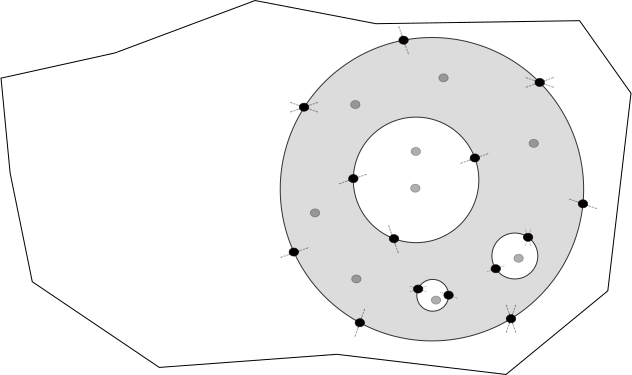
\includegraphics[width=1.0\textwidth]{figs/rdiv.pdf}
  \caption{Illustration of an $r$-division. A region $R$ of the graph $G$ is shown in
  grey with holes in white. Boundary vertices are shown as black circles, interior vertices are shown in
grey. Any edge passing through the Jordan curve goes through a boundary vertex as
indicated by the arrows.}
    \label{rdiv}
\end{figure}

\subsection{Monge property}
Given two ordered sets $A$ and $B$ and a distance function $d$, we say $d$ has the
\textit{Monge property} if for elements $u, v\in A$ and $x, y\in B$, where
$u\leq v$ and $x\leq y$, then:
\begin{align*}
  d(u,x)+d(v,y)\leq d(u, y)+d(v,x)
\end{align*}
An example of this is shortest paths distances between boundary vertices in planar graph
given all four boundary vertices lie on the infinite face. It states that the sum of
paths that do not cross is at most the sum of paths that do cross. Figure \ref{monge}
illustrates this. \\
Another implication of the property is that if we have found the $u$ that minimizes $d(u,y)$,
then for all boundary vertices $v$ that are on  counter clockwise path on the face $f$
(according to Figure \ref{monge}), then $d(v,x)\geq d(u,x)$. To see this, note that there
is a vertex $w$ on path from $u$ to $y$ that the path $v$ to $x$ must cross. Since
$d(u,y)\leq d(v,y)$, it implies that $d(u,w)\leq d(v,w)$. It is important that all
vertices are on the boundary of the face as it is otherwise not true (as indicated by
Figure \ref{monge2}). \\
The \textit{Monge matching problem} is finding the parent $p(v)\in A$ for all $v\in B$,
so that $d(p(v), v)\leq d(u,v)$ for any $u\in A$. The \textit{minimum Monge matching} is
the set of $(p(v), v)$.

\begin{figure}
  \centering
  \begin{subfigure}[b]{0.45\textwidth}
    \includegraphics[width=\textwidth]{figs/monge.pdf}
    \caption{Illustration of the Monge property in planar graphs. The sum of the distances
  when paths cross (in solid) are less than or equal to the sum of distances when paths
do not cross (in dashed lines).}
    \label{monge}
  \end{subfigure}
  \quad
  \begin{subfigure}[b]{0.45\textwidth}
    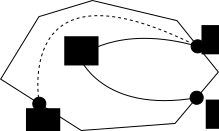
\includegraphics[width=\textwidth]{figs/monge2.pdf}
    \caption{A scenario where the Monge property does not hold, since paths
      do not cross. The shortest paths from $u$ are
      indicated by solid lines and a shorter path to $x$ is indicated by a dashed line.}
    \label{monge2}
  \end{subfigure}
\end{figure}

\subsection{Klein's multiple source shortest path}
Klein's multiple source shortest path \cite{klein2005multiple} is another useful tool for planar
graphs. Given a planar graph with nonnegative weight, we can construct a data structure
of size $O(n \lg n)$ that can answer queries of the following form in $O(\lg n)$ time:
For a source vertex $v$ and a vertex $s$ on the boundary of the infinite face, find the
shortest path from $v$ to $s$. This is especially useful to compute all pairs shortest paths between boundary
nodes in an $r$-division as it requires $O(r\lg r)$ time for a region $R$. \\
The idea is then to compute a shortest path tree $T$ rooted at
$s_i$ and then modifying the tree to get the shortest path tree rooted at the
neighbouring boundary vertex $s_{i+1}$. Using an efficient representation of dynamic
trees that allow operations to be done in amortized $O(\lg n)$ time is possible
\cite{tarjan2005self}\cite{henzinger1999randomized}. Any edge will then join the tree at
most once and leave the tree at most once. Since the graph is planar, we have $O(r)$ edges,
giving us the $O(r\lg r)$ running time. \\
The query idea is to use an Euler tour representation of the tree, called $T$, so we can
return the distance from a vertex $u$ to the root $r$ of the tree. Since we need the
correct version of the tree computed during preprocessing, we need a persistent data
structure that remembers changes, so we can recover any state of $T$.

\begin{figure}[h!]
  \centering
  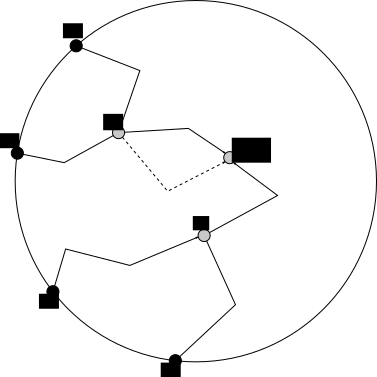
\includegraphics[width=0.6\textwidth]{figs/klein.pdf}
  \caption{Illustration of Klein's MSSP structure. The idea is two adjacent boundary
    vertices have almost identical shortest path trees. Computing shortest path trees
    $T_i$ clockwise
    around the face from $s_1$, we need only consider the \textit{differences} between
  the two trees. The dashed line is an impossible situation. Having computed the shortest
path tree rooted in $s_3$, $T_3$, where the shortest path to $v$ goes through $w$, it is
impossible for the shortest path tree rooted in $s_4$ to "cross" $T_3$ since it would
imply a shorter path from $w$ to $v$.}
    \label{klein}
\end{figure}

\subsection{FR-Djikstra}
A \textit{dense distance graph} or DDG is defined over a decomposition of a planar
graph. It is the non-planar graph $G'$ of $G$ where there is an edge $uv$ if both $u$ and
$v$ are boundary nodes with weight equal to the shortest path between the vertices.
Fakcharoenphol and Rao \cite{fakcharoenphol2006planar} gave an algorithm that can answer
distance queries between nodes in $O(\sqrt{n}\lg^2 n)$ after $O(n\lg^3 n)$ preprocessing.
The decomposition used in the algorithm is the result of applying a separator
recursively. For each level, the graph is split into "inside" and "outside" of the
separator. They then compute and store a MSSP for both inside and outside. At the same
time, we obtain the shortest paths between boundary nodes in the graph. Using Klein's
algorithm \cite{klein2005multiple}, this can be done in $O(n\lg n)$ time for each level.
The depth of the recursion is $O(\lg n)$, which means we can get preprocessing down to
$O(n\lg^2 n)$ time using $O(n\lg n)$ space. \\
After consutrcting the dense distance graph, it is possible to to compute a shortest path
tree $T$ in $G'$ that obey the Monge property. Using the Monge property, they can compute
$T$ in time linear to number of vertices in $G'$ which is significantly lower than the
number of vertices in $G$. Specifically, the graph is divided into bipartite graph that
all comply with the Monge property and then invoke a Djikstra-like algorithm that run in
time proportional to the number of vertices in $G'$.

\subsection{Additively weighted Voronoi diagrams}
When we find a Jordan curve which split the region $R$ into subregions $P$ and $Q$, we
define an \textit{additively weighted Voronoi diagram} from a vertex $u\in P$ and a hole
$h$ in $Q$. We write $VD(u,h)$ to denote the diagram. The sites of the Voronoi diagram
are the boundary vertices of the hole $h$. A vertex $v$ in the interior of $h$ belongs to
the Voronoi cell given by boundary node $s_i$ (site) if the distance from $u$ to $s_i$ plus the distance from $s_i$ to $v$ is less
than the same distance through any other boundary vertex. \\
The representation we are interested in is the one given by the dual $VD^*(u,h)$, where
each face in the primal graph (which we assume is fully triangulated) correspond to a
vertex in $VD^*$ and there is an edge in $VD^*$ whenever two faces share an edge in the
primal graph. We further contract edges in $VD^*$ incident to vertices of degree two.
This ensures that all vertices have degree three (faces that are incident to three
vertices of the primal graph which all belong to different sites in the Voronoi diagram
$VD$. Figure \ref{awvd} illustrates this. \\
\begin{figure}
  \centering
  \begin{subfigure}[b]{0.45\textwidth}
    \includegraphics[width=\textwidth]{figs/awvd1.pdf}
    \caption{Illustration of an additively weighted Voronoi diagram $VD(u,h)$. The hole
    $h$ is shown with boundary vertices in black, interior vertices in grey. Any shortest path
  from $u$ (not shown) to an interior vertex must go through the boundary vertex whose
cell the interior vertex belongs to.}
    \label{awvd1}
  \end{subfigure}
  \quad
  \begin{subfigure}[b]{0.45\textwidth}
    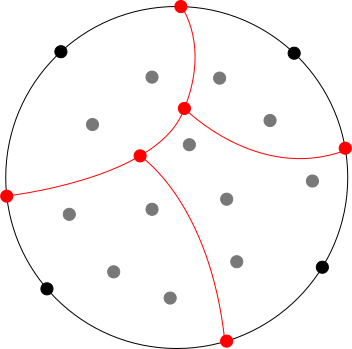
\includegraphics[width=\textwidth]{figs/awvd2.pdf}
    \caption{Illustration of the representation we are after $VD^*(u,h)$. The vertices of
      $VD^*$ are the intersection of edges of $VD$ with degree three. The diagram $VD^*$
    is given by red vertices and red edges.\\ \\}
    \label{awvd2}
  \end{subfigure}
  \label{awvd}
\end{figure}
Note that we can represent $VD^*$ using $O(\sqrt{r})$ as each hole has $r$ vertices and
$\sqrt{r}$ boundary vertices. The number of vertices in $VD^*$ is $O(\sqrt{r})$ as we
only get another vertex of degree three whenever we add another boundary vertex. Since
$VD^*$ is also planar, it has $O(\sqrt{r})$ edges.

\newpage
\section{Related work}\label{survey}
Distance oracles were introduced by Thorup and Zwick \cite{thorup2005approximate} as a
faster alternative to the SSSP and APSP algorithms. They proposed an approximate distance
oracle, which was later the inspiration for Hermelin et al. when they introduced distance
oracles for vertex-labeled graphs. \\
Hermelin et al. \cite{hermelin2011distance} proposed several results for approximate
distance oracles. In the first result, they give a vertex-labeled distance oracle of
expected size $O(kn^{1+1/k})$ with a stretch of $(4k-5)$ and query time $O(k)$. This can
be constructed in $O(kmn^{1/k})$ time. The data structure is an adaption of Thorup and
Zwick's distance oracle \cite{thorup2005approximate}. \\
In another result, they give a distance oracle which depend on both $n$ and $\ell$. This has
expected size $O(knl^{1/k})$ with query time $O(k)$, but with an exponential stretch of
$(2^k-1)$. This is constructed in $O(kmn^{k/(2k-1)})$. \\
In their third result, they give an oracle capable of handling label changes. This has
expected space $O(kn^{1+1/k})$, stretch $(2\cdot3^{k-1}+1)$, query time $O(k)$ and
handles label changes in $O(kn^{1/k}\lg \lg n)$. \\
\\
Chechik \cite{chechik2012improved} improved the latter two results. Namely, she managed to
reduce the stretch from exponential down to polynomial. She showed two theorems that can
be stated as follows:
\begin{thm}\label{chech1}
  There is a vertex-labeled distance oracle
of size $O(kn\ell^{1/k})$, stretch $(4k-5)$  and query time $O(k)$, which can be
constructed in $O(m\cdot \min\{n^{k/(2k-1)}, \ell\})$.
\end{thm}
\begin{thm}\label{chech2}
  There is a dynamic vertex-labeled distance oracle capable of handling label changes in
$\tilde{O}(n^{1/k})$ time with stretch $(4k-5)$ and space $\tilde{O}(n^{1+1/k})$. It has
query time $O(k)$ and can be constructed in $O(kmn^{1/k})$.
\end{thm}
\noindent
However, the focus of this thesis is on exact distance oracles and the approaches used to
approximate distances are often not applicable to obtain exact distance oracles. Below, we outline results for exact distance oracles for both graphs that are labeled and
graphs that are not labeled.

\subsection{The general case}


\subsection{The planar case}\label{cohenplanar}
Given a directed planar graph $G$ with both positive and negative weighted edges, Klein
et al. \cite{klein2010shortest} gives an algorithm with $O(n\lg^2 n)$ preprocessing and
$O(n)$ space that can answer shortest paths. 



Cohen-Addad et al. \cite{cohen2017fast} introduced a (non vertex-labeled) distance
oracle in planar digraphs that required subquadratic space and could answer exact distance queries in
$O(\lg n)$ time. This was the first result to achieve polylogarithmic query time, as previous
results required query time polynomial in $n$ or could only return approximate distances.
This result was later improved in \cite{gawrychowski2017better} from using $O(n^{5/3})$
space to $O(n^{3/2})$ space. They also improved the tradeoff for any space $S\in [n,n^2]$.
That is, for $S\in [n, n^{3/2}]$, they give an oracle with query time
$\tilde{O}(n^{3/2}/S)$. For $S\in [n^{3/2}, n^2]$, they give an oracle with query time
$O(\lg n)$. \\
\\
TODO:
\begin{itemize}
  \item Recursive decomposition using Jordan curves.
  \item Voronoi diagrams
  \item Distances stored
  \item Point location approach
\end{itemize}
We give two exact vertex-labeled distance oracles for planar graphs in \ref{exactPlanar}.

\begin{table}[H]
  \footnotesize
  \centering
  \begin{tabular}{c | c | c | c | c}
    Reference & Dir. & Preprocessing & Space & Query \\
    \hline\hline
    This & D & $O(n^2/\ell{1/3})$ & $O(n\ell^{2/3})$ & $O(\ell^{1/3})$ \\
    \hline
    This & D & TODO & $O(n^{3/2})$ & $O(\text{polylog}(n))$ \\
    \hline
    Mozes et al. \cite{mozes2015efficient} & U & $O(\varepsilon^{-2}n\lg^3 n)$ & $O(\varepsilon^{-1}n\lg n)$ &
    $O(\lg \lg n + \varepsilon^{-1})$ \\
    \hline
    Mozes et al. \cite{mozes2015efficient} & D &
    $O(\varepsilon^{-2}n\lg^3 n\lg (nN))$ & $O(\varepsilon^{-1}n\lg n \lg(nN))$ & $O(\lg
    \lg n \lg \lg (nN) + \varepsilon^{-1})$ \\
    \hline
    Li et al. \cite{li20131+} & U & $O(\varepsilon^{-1}n\lg^2 n)$ & $O(\varepsilon^{-1}n\lg n)$ & $O(\varepsilon^{-1}\lg
    n \lg \Delta)$
  \end{tabular}
  \caption{Results for vertex-labeled distance oracles in planar graph. All results are
  for connected graphs. All results but those introduced in this thesis are
$(1+\varepsilon)$ stretch results. The letters 'U' and 'D' is for undirected and directed
graphs respectively. The 'N' is the maximum arc length and $\Delta$ is the hop-diameter
of the graph.}
  \label{planarresults}
\end{table}

\newpage
\section{Exact Oracles in Directed Planar Graphs}
\label{sec:sota}
Previous works have given exact distance oracles for directed planar graphs of size
$O(n^{5/3})$ with query time $O(\lg n)$ \cite{cohen2017fast}. This was improved recently
to use $O(n^{3/2})$ space \cite{gawrychowski2017better}. TODO: Other results. \\
\\
We cannot directly adapt the approach used in \cite{cohen2017fast} and \cite{gawrychowski2017better} to work
for the vertex-labeled case as it requires us to know the "target" vertex. However,
depending on $\ell$, we can construct the following distance oracle:\\
\\
\textit{Data structure}. Given the graph $G$ and a number of labels $\ell$ with
$\varepsilon_1 = O(\sqrt{n})$ and $\varepsilon_2=O(\lg n)$, if $\ell\in
[1, \varepsilon_1]$, simply store the matrix of all shortest paths for all nodes to all
labels in the graph. \\
If $\ell\in [n-\varepsilon_2, n]$, we use the same approach as in
\cite{gawrychowski2017better}. \\
If $\ell\in (\varepsilon_1, n-\varepsilon_2)$, we construct an $r$-division with $r=\ell^{2/3}$. For each node within a region, store distances to all
labels in that region in a hash table. For each boundary node, store distances to all
labels outside the region. \\
\\
\textit{Query}. For the query $Q(v, \lambda)$, if $\ell\in[1, \varepsilon_1]$, we simply look up the distance in the matrix
in constant time. \\
If $\ell\in [n-\varepsilon_2, n]$ we compute all distances from node $v$ to the given label (note
that there cannot be more than $\lg n$ nodes with this label. Pick the minimal distance
using $O(\lg n\lg n)$ time. \\
If $\ell\in (\varepsilon_1, n-\varepsilon_2)$ we check if $\ell$ exists in the region of $v$. If so,
we can look up the distance in the hash table
stored for $v$. We also run over all boundary nodes and return the minimal distance
$d(v,w)+d(w,\lambda)$ for some boundary node $w$ in
$O(\sqrt{r})=O(\ell^{1/3})$ time. \\


\section{Recursion}
We can improve the space slightly if we construct the $r$-division recursively. This will
yield space:
\begin{align*}
  \sum_{i=1}^{lg_{n/r}(n)} \left(\frac{n}{r}\right)^i
  \sqrt{r\left(\frac{r}{n}\right)^{i-1}} \min
  \left\{\ell,\left(n-r\right)\left(\frac{r}{n}\right)^{i-1}\right\}
\end{align*}



\section{Remarks}
Klein's multiple source shortest path \cite{klein2005multiple} is one \\
FR-Djikstra \cite{fakcharoenphol2006planar}\\
Nearest neighbour searches in $\lg n$ time. \\
Exploiting Monge property


\newpage
\section{Dynamic Oracles in Directed Planar Graphs}\label{dynamicPlanar}
In this chapter we show how to construct a dynamic distance oracle to handle
edge weight changes, edge insertion and deletions in in amortized $\tilde{O}(n^{2/3})$
time. We also show how to extend the oracle from Section
\ref{oracle2} to support label changes in expected $O(1)$ time.

\subsection{A dynamic oracle supporting edge weight updates}\label{oracle3}
We now give a simple dynamic distance oracle using the same approach as in FR-Djikstra that can support edge weight changes, edge
insertions and deletions when no updates will violate the planar embedding of $G$. We
show the following theorem:
\begin{thm}\label{thm4}
  There is a data structure that can be preprocessed in $O(n\lg n)$ using $O(n\lg n)$
  space that can update edge weights, insert and delete edges in in amortized
  $O(n^{2/3}\lg^{5/3} n)$. It answer queries $Q(u,\lambda)$ in
  $\tilde{O}(\min\{\text{size}(\lambda)\cdot n^{2/3}, n\})$ time.
\end{thm}
\indent \textit{Data structure}.
Given a planar graph $G$ with non-negative edge length, We construct an $r$-division and maintain a dense distance graph of all the pieces. As
described in Section \ref{frdjikstra}, we also need to construct the Monge heaps. \\
\\
\indent \textit{Edge weight update}.
We simply update the weight of the edge and, if necessary, recompute the dense distance graph in which
the modified edge is. \\
\\
\indent \textit{Edge deletion}.
A deleted edge will always happen entirely within a single piece $P$, so we simply remove
the edge and if necessary, we recompute the dense distance graph of $P$. \\
\\
\indent \textit{Edge insertion}.
There are two cases whenever we insert an edge. If the inserted edge is in a single piece
$P$, we simply insert it. If the endpoints, $u$ and $v$, of the inserted edge belong to two different
pieces, it will violate the property of an $r$-division. That is, any edge going out of
the piece, must go through a boundary vertex. However, we can overcome with by making $u$
a boundary vertex of the piece it belongs to. This will not increase the number of holes,
and we recompute the dense distance graph of $P$ if needed. \\
\\
\indent \textit{Query}. To answer the query $Q(u,\lambda)$, we use Djikstra variant
described in Section \ref{frdjikstra}. Since this algorithm answers the query $Q(u,v)$,
we need to do $size(\lambda)$ iterations after the FR-Djikstra step. We answer the query
$Q(u,v)$ by computing distances from $u$ to all boundary vertices in its piece $P_u$.
When we have completed the fast Djikstra step, we have distances to the boundary vertices
of the piece, $P_v$, that $v$ belongs to, and we can compute distances from the boundary
vertices of $P_v$ to $v$. If $P_u=P_v$, then we also compute the shortest path from $u$
to $v$ within the piece and we pick the shortest one. \\
Note that we can use reuse the relaxed DDG after the Djikstra step to find distances to
all vertices with label $\lambda$. In case $\text{size}(\lambda)$ is $\Omega(n^{1/3})$, we simply run Henzinger et al.
\cite{henzinger1997faster} algorithm the original graph $G$ and pick the minimal distance
found to a vertex with label $\lambda$.

\subsubsection{Analysis}
\textbf{Preprocessing}.
We can compute an $r$-division in $O(n)$
time. We then
construct a dense distance graph, that is, we construct the graph where each edge $uv\in
E$ has weight equal to $\delta(u,v)$ and $u$ and $v$ are both boundary nodes. We use
Klein's multiple source shortest path algorithm \cite{klein2005multiple} to compute DDG's
for each region of an $r$-division. For each region $R$ with $r$ nodes, we use $O(r\lg
r)$ preprocessing to compute distances $\delta(u,v)$ in $O(\lg r)$ time where either $u$
or $v$ is a boundary node. Since each region has $O(\sqrt{r})$ boundary nodes and $O(1)$
holes, we can compute all distances in $O(r\lg r)$ time. Since there are $O(n/r)$
regions, this yields a total running time of $O(nr\lg r/r)=O(n\lg r)$ to construct the
dense distance graph. Using the implementation of Kaplan et al.
\cite{kaplan2012submatrix}, we can construct the Monge heaps in $O(n\lg n)$ time.\\
\\
\textbf{Space}. The dense distance graph has $O(n/\sqrt{r})$ vertices and $O(r)$ edges
per piece, which is $O(n)$ edges overall. So representing the dense distance graphs takes
$O(n)$ space. Each vertex occurs in $O(\lg n)$ different heaps and each edge is in one
data structure. The Monge heaps dominates the total space usage which is $O(n\lg n)$
\cite{kaplan2012submatrix}. \\
\\
\textbf{Updates}.
 Since we recompute the $r$-division after we have
done an order of $\sqrt{r}$ operation, we know that each piece cannot at any time have
more than $O(r)$ edges and $O(\sqrt{r})$ boundary vertices. An amortized analysis over
all $\sqrt{r}$ operations gives us $O(\frac{n+n\lg r}{\sqrt{r}})=O(n\lg r/\sqrt{r})$ for
each graph modification. \\
\\
\textbf{Query}. For each query $Q(u,v)$, we know that each FR-Djikstra step, i.e. computing
the shortest paths in the dense distance graph, requires $\tilde{O}(n/\sqrt{r})$ time.
Computing distances within a piece requires $O(r)$ time using the algorithm of Henzinger
et al. \cite{henzinger1997faster}. Thus the total time for the query $Q(u,\lambda)$ is
$\tilde{O}(\text{size}(\lambda)\cdot r+n/\sqrt{r}))$. \\
In the case that $\text{size}(\lambda)$ is $\Omega(n^{1/3})$, we run the SSSP algorithm
of Henzinger et al. in $O(n)$ time. \\
\\
If we pick $r=n^{2/3}$, we get Theorem \ref{thm4}, but we can pick a smaller $r$ to obtain
slightly better query times at the cost of worse update times.

\subsection{A dynamic oracle supporting label changes}\label{oracle4}
Recall the oracle described in Section \ref{oracle2}. We now give an oracle that can
handle label changes in $O(1)$ time. Namely, we show the following theorem if we assume
that there are no more than $O(\sqrt{n})$ labels of polynomial size and a label change
does not change this:
\begin{thm}\label{thm3}
  There is an oracle of requiring preprocessing time $O(n^{3/2})$ of size $O(n^{3/2})$ that
  can answer distance queries in $O(\text{polylog}(n))$ time. Furthermore, it can handle
  label changes in expected amortized $O(1)$ time.
\end{thm}
\textit{Data structure}.
We are given a directed planar graph $G$ with non-negative edge length. The data structure is constructed almost the same way as the one described in Section
\ref{oracle2}, but we modify the hash table used in it and add another one. The added
hash table is used for a simple lookup of what label a vertex has. That is, we use the
vertex number as key and store the label as the information. Note that we can pick our
hash function to avoid any collision (e.g. vertex $v$ \texttt{mod} $n$). Call this hash
table for $h_1$. \\
We also store another hash table keeping track of all vertices with a given label as in
the static case. That is, given a label $\lambda$, we return all vertices with $\lambda$.
We call this hash table for $h_2$. \\
\\
\indent\textit{Update}.
Every time we make a label change, we need to lookup the label in $h_1$ and change
it to the new one. However, since we also need to be able to retrieve all vertices given some label
$\lambda$ (which we obtain from $h_2$) in the query, we need the other hash table to adjust accordingly. This means
removing the vertex from the hash table and inserting in its new location in the hash table.

\subsubsection{Analysis}
Preprocessing, space and query time follows from the analysis in Section
\ref{oracle2analysis} as it is the same construction. \\
However, we need to analyse the update time. We can easily construct $h_1$ in $O(n)$ time
requiring $O(n)$ space, and since each bucket contains a single element, deletion of the
record  can be done in $O(1)$ time and insertion (of a new label) can be done $O(1)$ time
too. \\
\\
Constructing $h_2$ requires a little more. Each bucket can be expected to
have $n/\ell$ elements, but in worst case they can be up to $O(n)$ in size. Therefore we
need a \textit{dynamic perfect hashing} scheme that supports $O(1)$ lookup and
amortized expected insertion and deletion in constant time. Dietzfelbinger et al.
\cite{dietzfelbinger1994dynamic} introduced an algorithm achieving this. The idea is to use a
primary hash function to construct buckets containing all vertices with the same label.
These buckets are dynamic arrays. We use hashing with chaining for the vertices in each bucket to ensure we have expected lookup in $O(1)$ time. The algorithm keeps track of how many elements are in
each bucket and we refer to these numbers as $b_i$. Each bucket is assigned $s_i$ space,
where $s_i=2b_i$. For each bucket, there is a specified threshold $t_i=(1+c)b_i$ (in this
case, we use $c=1$). When $b_i$ exceeds $t_i$ or falls below
$t_i/(1+2c)$, the array is destroyed and a new (larger or smaller) array is created and
we rehash all elements of the bucket into it in $O(n)$ time. \\
Now lookup can easily be done in $O(1)$ time, since we lookup the label in $h_1$ in
$O(1)$ time. Given the label, we can locate the vertex in $h_2$ in $O(1)$ time as well.
Deletion and insertion (which is what a label change requires) in $h_1$ is done in
expected $O(1)$
time. When we want to delete an element $x$ from $h_2$, we first perform a lookup of $x$
and mark the slot as empty as well as decrementing $b_i$ by one. For insertion, we can
add $x$ to its proper place in expected $O(1)$ time and we increment $b_i$ by one. \\
Since we rarely need to rehash elements into a dynamic array, we achieve the expected amortized
constant update time. First we need to show that we can expect any 'chain' in the array
will have constant size. We hash $b_i$ elements uniformly at random into a table of size
$s_i=2b_i$, thus any chain is expected to have $1/2$ elements - also called the load
factor $\alpha$. When $\alpha$ is $O(1)$, we can also expect constant search, insertion and
deletion \cite{cormen2009introduction}. \\
The space taken by the hash table is $O(n)$, which can be seen by inspecting the size of
each array. The arrays have size $s_i$ which all have size $O(b_i)$, so we get space $S$ is
\begin{align*}
  S&=O\left(\sum_i s_i\right) \\
   &=O\left(\sum_i b_i\right) \\
   &=O(n) \comment{As $\sum_i b_i = n$}
\end{align*}
This will yield the result in Theorem \ref{thm3}.

\newpage
\section{Concluding remarks}\label{conclusion}
The goal of this thesis was to explore vertex-labeled distance oracle in planar directed
graphs. We have given two oracles in the static setting. One described in Section
\ref{oracle1} which is simpler than the
other, but still has its applications when the number of labels is low, i.e below
$\sqrt{n}$, or when the desired space allocation is $o(n^{3/2})$. The other oracle in
Section \ref{oracle2} beats
the space-query product of the trivial solution and it matches the best theoretical
trade-offs for distance oracles in planar graph that are not vertex-labeled. Even though
it does not work for all distributions of $L$, it arguably works for many realistic
cases. \\
We also gave two distance oracles in the dynamic setting. The first result in Section
\ref{oracle3} tried to match the
trade-offs given by the works based upon FR-Djikstra. Previous works have not been able
to reduce the trade-off of FR-Djikstra with more than a factor of $O(\lg^2\lg n)$, but
have been able to produce oracles that extend it with other operations with the same
update times as well as handling negative edge-lengths. We have shown it can be extended to vertex-labeled planar graphs. The
oracle in Section \ref{oracle4} supports the classic update in vertex-labeled graph - the
label change. We managed to do this in expected constant time, though without the
assumption on the distribution of $L$, the update time will suffer.

\subsection{Reflections and future works}
The obvious improvement would be remove the assumption on the distribution of $L$. I
tried different strategies. My first observation was that we wanted, given a query
$Q(u,\lambda)$, to find the nearest $\lambda$-labeled vertex to $u$. This boils down to
the nearest neighbor problem in planar graphs (known by many names). If we could be able to construct a data structure
of size $O(n^{3/2})$ that could answer this problem in $O(\lg n)$ time, the overall time
bounds would not be affected. However, it seemed that for a single label, this would
require linear space, which would add up to $O(n\ell)$ space for all labels. Most
landmark based methods did not seem to help either. A whole line of work is dedicated to
nearest neighbour search in general metrics
\cite{krauthgamer2004navigating}\cite{krauthgamer2005black}\cite{karger2002finding}\cite{plaxton1999accessing}\cite{beygelzimer2006cover}\cite{cole2006searching}.
However, all of them are approximate results and often work under certain conditions
(growth-restricted, low doubling dimension etc.). One might hope to uncover an exact NNS
structure or even one that can return the $k$ nearest neighbours for
$k=O(\text{polylog}(n))$ as this would be sufficient to fix the gap in the distance
oracle. \\
Besides mending current results, one could research if the results could extend to related
families of graphs. In particular, the $O(n)$-separable graphs, bounded genus graphs,
graphs with bounded treewidth.


\newpage
\addcontentsline{toc}{section}{References}
\bibliography{report}
\bibliographystyle{ieeetr}

\newpage
\appendix
%\section{Missing proofs}
\subsection{$VD^*$ is a tree}
Kyl det ind

\subsection{Point location in $VD^*$}
Throw it in

\subsection{Dynamic hashing?}


\end{document}
